% Created 2020-03-24 Tue 14:37
% Intended LaTeX compiler: pdflatex
\documentclass[11pt]{article}
\usepackage[utf8x]{inputenc}
\usepackage[T1]{fontenc}
\usepackage{graphicx}
\usepackage{grffile}
\usepackage{longtable}
\usepackage{wrapfig}
\usepackage{rotating}
\usepackage[normalem]{ulem}
\usepackage{amsmath}
\usepackage{textcomp}
\usepackage{amssymb}
\usepackage{capt-of}
\usepackage{hyperref}
\usepackage{minted}
\author{Jakub Zárybnický (xzaryb00@stud.fit.vutbr.cz)}
\date{\today}
\title{Konstrukce fylogenetických stromů}
\hypersetup{
 pdfauthor={Jakub Zárybnický (xzaryb00@stud.fit.vutbr.cz)},
 pdftitle={Konstrukce fylogenetických stromů},
 pdfkeywords={},
 pdfsubject={},
 pdfcreator={Emacs 26.3 (Org mode 9.1.9)}, 
 pdflang={Czech}}
\begin{document}

\maketitle

\section{Viacnásobné zarovnanie sekvencie cytochromu C a základná fylogenetická analýza}
\label{sec:org9aec594}
Stiahnite si aminokyselinové sekvencie nasledovných organizmov z \href{http://www.ncbi.nlm.nih.gov/protein/}{NCBI} a
uložte ich do jedného multifasta súboru:

\begin{itemize}
\item Equus caballus (NP\(_{\text{001157486.1}}\))
\item Homo sapiens (NP\(_{\text{061820.1}}\))
\item Bos taurus (NP\(_{\text{001039526.1}}\))
\item Gallus gallus (NP\(_{\text{001072946.1}}\))
\item Canis lupus (AEP27248.1)
\item Sus scrofa (NP\(_{\text{001123442.1}}\))
\item Pan troglodytes (NP\(_{\text{001065289.1}}\))
\item Taeoniopygia guttata (NP\(_{\text{001137145.2}}\))
\item Novosphingobium sp. PP1Y (WP\(_{\text{013831814.1}}\))
\end{itemize}

Sekvencie importujte do programu MEGA a analyzujte:
\begin{itemize}
\item Kliknite File->Open a File/Session, How would you like to open this fasta
file - kliknite Align, potom z menu Alignment exploreru vyberte Alignment ->
Align by ClustalW (ak sedíte v sudom stĺpci), resp. Muscle (ak sedíte v lichom
stĺpci). \textbf{Vyšiel susedovi rovnaký alignment?}
\begin{itemize}
\item V několika pozicích se Muscle a ClustalW liší, v umístěni gaps
\end{itemize}
\item Vizuálne porovnajte jednotlivé zarovnané sekvencie. *Ktorá zo
sekvencií sa zarovnala vzhľadom k ostatným nesprávne/je vysoko
divergentná vzhľadom k ostatným? Do akej skupiny organizmov patrí?*
\begin{itemize}
\item Novosphingobium sp. PP1Y je jediná viditelně odlišná, jedná se o proteobakterii
\end{itemize}
\item \textbf{V koľkých pozíciách sa líšia zvyšné sekvencie?}
\begin{itemize}
\item Zběžně jsem napočítal 14 pozic
\end{itemize}
\item V Alignment exploreri vyberte v menu Data->Export alignment->Mega
format a uložte.
\item Zatvorte Alignment explorer (alignment už znova nemusíte ukladať)
\item Vytvorte v programe Mega jednoduchú fylogenetickú analýzu - ak ste
v sudom stĺpci, použite algoritmus NJ, ak ste v lichom stĺpci,
použite Maximum Parsimony (Phylogeny->Construct NJ/Maximum
parsimony).
\end{itemize}

Pre algoritmus \textbf{NJ} použite:
\begin{itemize}
\item Model/Method: Equal Input Model
\item Gaps/Missing Data Treatment: Partial deletion
\end{itemize}

Pre algoritmus \textbf{Maximum Parsimony} použite:
\begin{itemize}
\item Gaps/Missing Data Treatment: Partial deletion
\end{itemize}

Ostatné parametre ponechajte implicitné. V TreeExploreri sa Vám zobrazí
vygenerovaný fylogenetický strom. Zvoľte v menu TreeExploreru Subtree->Root a
kliknite na vetvu Novosphingobium.  Týmto strom "zakoreníte" a označíte
Outgroup.

\begin{itemize}
\item Zhoduje sa topológia stromov vytvorených pomocou MP a NJ? V čom sa líšia?
Diskutujte s Vašimi susedmi výsledky.
\begin{itemize}
\item Původně jsem psal, že stromy jsou stejně, ale to musela být chyba. "Original
tree" se liší značně - \emph{Canis lupus} je podle MP nejméně podobný
ostatním. "Bootstrap consensus tree" už je podobnější, ale pořád se liší ve
stromu kopytnatců, kde prase je blíže buď koni (v MP), nebo turovi (v NJ).
\end{itemize}
\item Vypátrajte české/slovenské názvy skúmaných organizmov. Korešponduje vzniknutý
fylogenetický strom s ich fenotypom?
\begin{itemize}
\item Ne úplně - kopytnatci jsou ve výsledné topologii správně blízko, ale jsou blíže
ptákům (zebřička a kur) než člověku nebo šimpanzovi.
\end{itemize}
\end{itemize}

\begin{center}
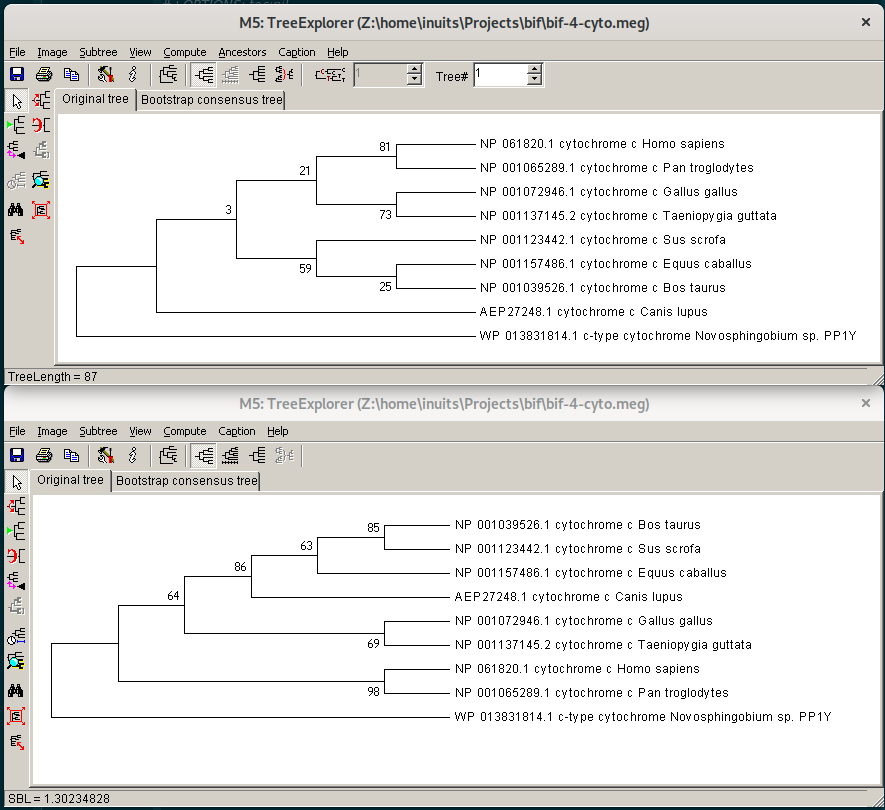
\includegraphics[width=1.2\linewidth]{./bif-4-cytotree.png}
\end{center}

\section{Fylogenetická analýza človeka s príbuznými druhmi}
\label{sec:org76a6dc4}
Zostavte si jednoduchý dataset (multifasta) pozostávajúci z DNA sekvencií
mitochondrial d-loop nasledovných druhov, ktoré si stiahnite z \href{http://www.ncbi.nlm.nih.gov/nuccore/}{NCBI}. Ako popis
sekvencií v multifasta súbore použite české/slovenské názvy organizmov.
\begin{itemize}
\item Pongo abelii (FR717938.1) alias orangutan
\item Pan troglodytes (GU136845.1) alias šimpanz
\item Homo sapiens (HM009355.1) alias človek dnešného typu
\item Gorilla graueri (AF050738.1) alias gorila
\item Homo sapiens neanderthalensis (FM866397.1) alias neandertálec
\end{itemize}

Sekvencie analyzujte pomocou programu MEGA nasledovne:
\begin{itemize}
\item Kliknite File->Open a File/Session, How would you like to open this
fasta file - kliknite Align, potom z menu Alignment exploreru
vyberte Alignment -> Align by ClustalW.
\item V Alignment exploreri vyberte v menu Data->Export alignment->Mega
format a uložte.
\item Zatvorte Alignment explorer (alignment už znova nemusíte ukladať)
\item Analyzujte zarovnanie pomocou fylogenetickej analýzy s využitím
bootstrapingu. Ak sedíte v lichom stĺpci, použite Phylogeny ->
Construct/Test Maximum likelihood tree, ak sedíte v sudom stĺpci,
použite Phylogeny -> Construct/Test Neighbor-Joining tree a
nastavte parametre:

\begin{itemize}
\item Test of phylogeny: Bootstrap method
\item No. of Bootstrap Replications: 1000
\item Model/Method: Kimura 2-parameter model
\item Gaps/Missing Data Treatment: Partial deletion
\end{itemize}

Ostatné parametre ponechajte implicitné. V TreeExploreri sa Vám
zobrazí vygenerovaný fylogenetický strom a consensus strom.

\item Majú obidva stromy rovnakú topológiu? Čo prezrádzajú bootstrapové hodnoty? Čo
je najpodobnejšie človeku? Majú na základe získaného stromu neandertálec a
človek dnešného typu priameho spoločného predka?
\begin{itemize}
\item Stejnou topologii nemají, ML a NJ se liší v zařazení orangutana (na společné
větvi se šimpanzem, nebo s člověkem/neandertálcem).
\item Bootstrapová hodnota ukazuje, kolikrát byl takový podstrom sestavený při
převzorkování z X iterací - vynechání jednoho sloupce a sestavení stromu z
upravených dat.
\item Nejpodobnější člověku je neandertálec, nejspíše přímého předka mají.
\end{itemize}
\end{itemize}
\end{document}